\subsection{Боксплот Тьюки}
	\begin{figure}[H]
		\centering
		\begin{tabular}{ccc}
			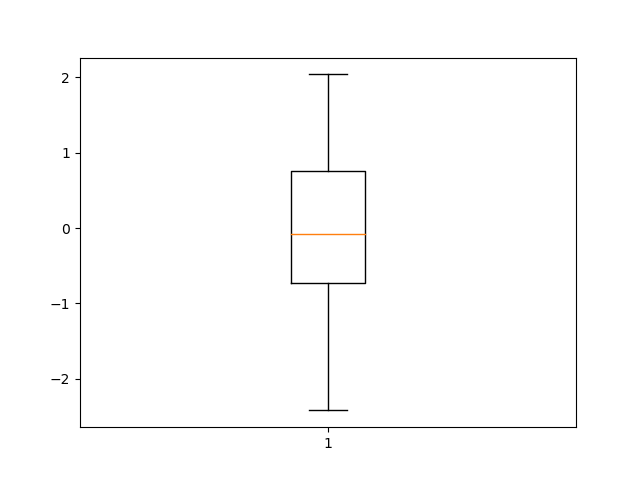
\includegraphics[width=55mm, height =0.25\textheight]{pics/n20.png}
			&
			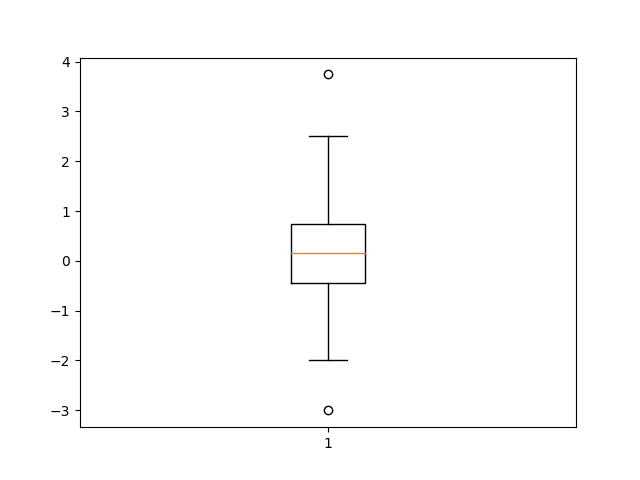
\includegraphics[width=55mm, height =0.25\textheight]{pics/n100.png}
		\end{tabular}
		\caption{Нормальное распределение}
		\label{fig:normal}
	\end{figure}

	\begin{figure}[H]
		\centering
		\begin{tabular}{ccc}
			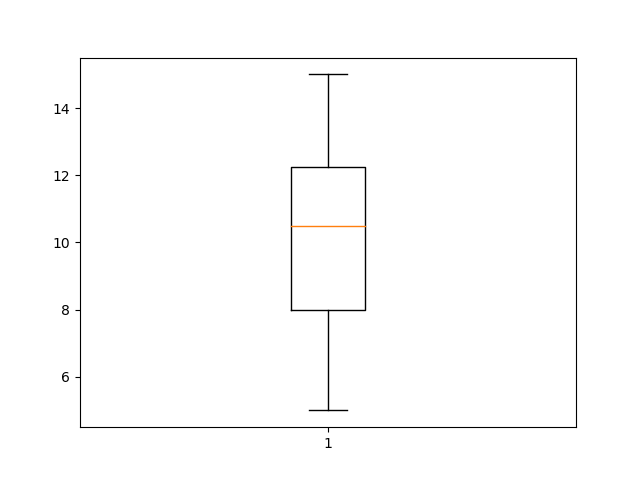
\includegraphics[width=55mm, height =0.25\textheight]{pics/c20.png}
			&
			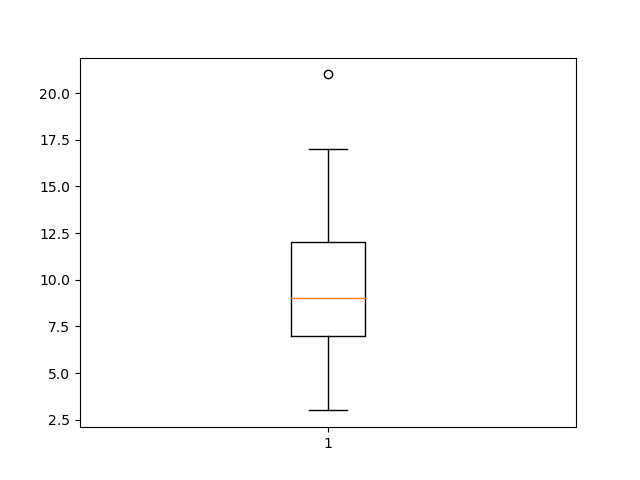
\includegraphics[width=55mm, height =0.25\textheight]{pics/c100.png}\
		\end{tabular}
		\caption{Распределение Коши}
		\label{fig:cauchy}
	\end{figure}
	

	\begin{figure}[H]
		\centering
		\begin{tabular}{ccc}
			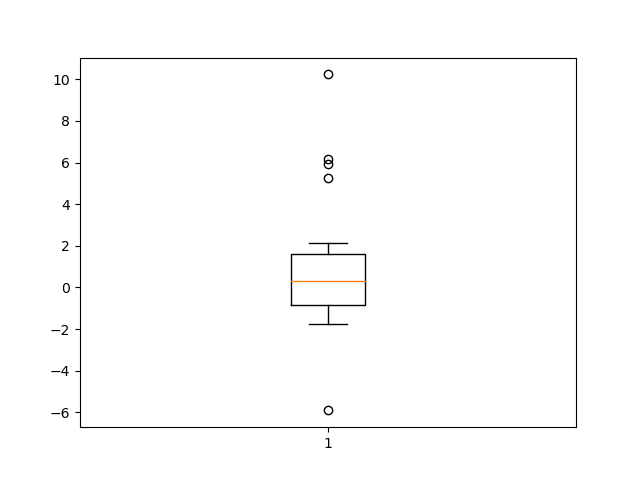
\includegraphics[width=55mm, height =0.25\textheight]{pics/l20.png}
			&
			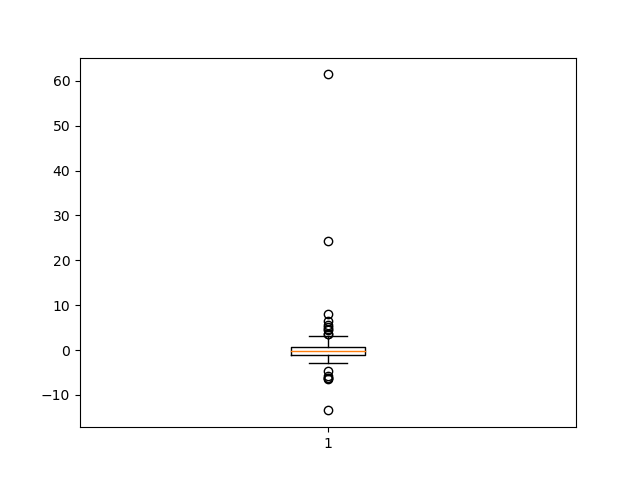
\includegraphics[width=55mm, height =0.25\textheight]{pics/l100.png}\
		\end{tabular}
		\caption{Распределение Лапласа}
		\label{fig:laplace}
	\end{figure}


	\begin{figure}[H]
		\centering
		\begin{tabular}{ccc}
			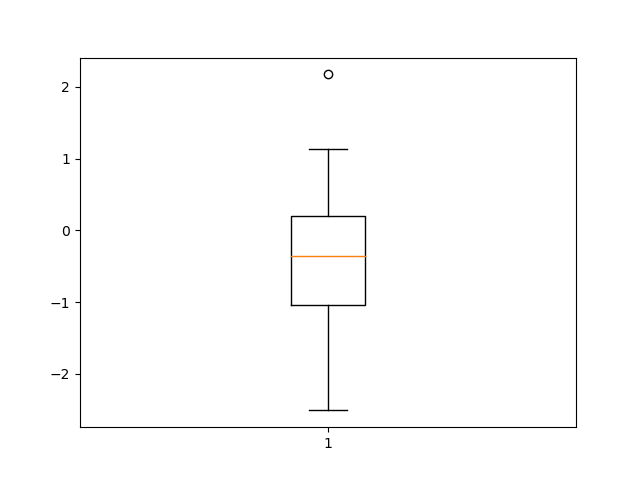
\includegraphics[width=55mm, height =0.25\textheight]{pics/p20.png}
			&
			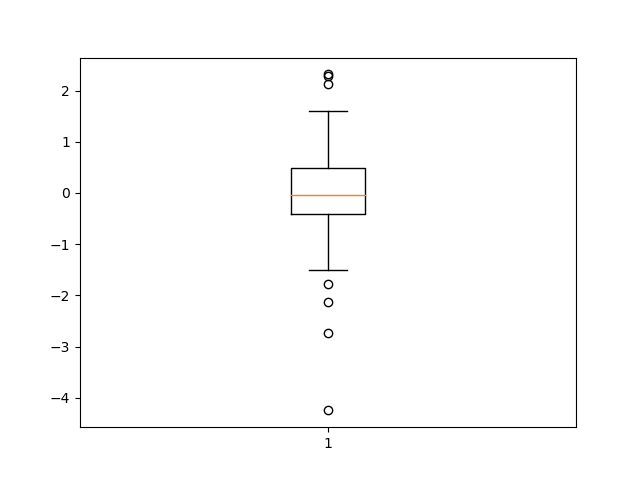
\includegraphics[width=55mm, height =0.25\textheight]{pics/p100.png}
		\end{tabular}
		\caption{Распределение Пуассона}
		\label{fig:poisson}
	\end{figure}


	\begin{figure}[H]
		\centering
		\begin{tabular}{ccc}
			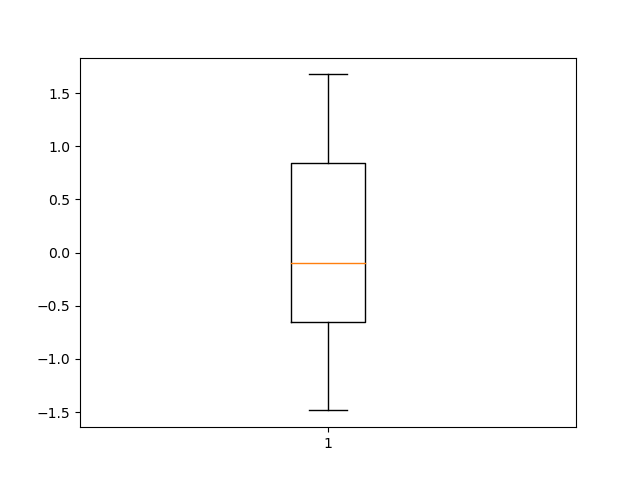
\includegraphics[width=55mm, height =0.25\textheight]{pics/u20.png}
			&
			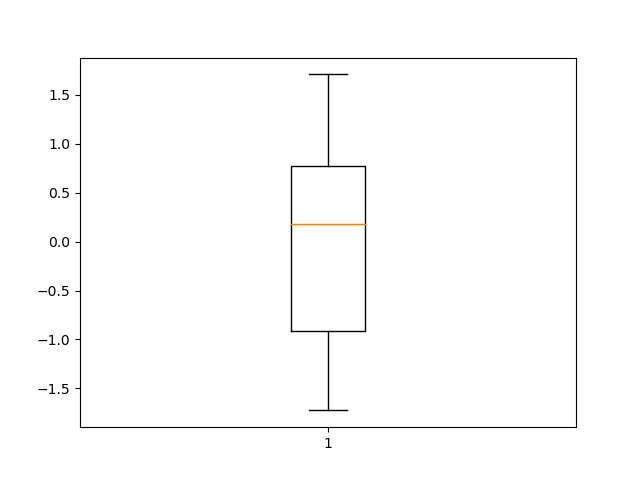
\includegraphics[width=55mm, height =0.25\textheight]{pics/u100.png}
		\end{tabular}
		\caption{Равномерное распределение}
		\label{fig:uniform}
	\end{figure}

\subsection{Доля выбросов}
	\begin{table}[H]
		\centering
		\begin{tabular}[t]{lr}
			\hline
			Выборка   &      Доля выбросов		\\
			\hline
			Normal n=20   	&	0.06 				\\
			Normal n=100   	&  	0.05		\\
			Cauchy n=20 	& 	0.15  				\\
			Cauchy n=100	&  	0.16 		\\
			Laplace n=20		& 	0.08  			\\
			Laplace n=100	&  	0.07 		\\
			Poisson n=20	&	0.02 				\\
			Poisson n=100	&	0.01 				\\
			Uniform n=20	&	0 				\\
			Uniform n=100	&	0 				\\
			\hline
		\end{tabular}
		\caption{Доля выбросов}
		\label{tab:normal}
	\end{table}

\subsection{Теоретическая вероятность выбросов}
	\begin{table}[H]
		\centering
		\begin{tabular}[t]{lrrrrr}
			\hline
			Распределение   &      $Q_1^T$	& $Q_3^T$ & $X_1^T$ & $X_2^T$ & $P_B^T$	\\
			\hline
			Нормальное распределение 	& -0.674& 0.674 & -2.698 	&  2.698 	& 0.007 \\
			Распределение Коши 			& -1	& 1		&  -4		& 4			& 0.156 \\
			Распределение Лапласа 		&-0.490	& 0.490	& -1.961	& 1.961		& 0.063\\
			Распределение Пуассона 		& 8		& 12	& 2			& 18		& 0.008 \\
			Равномерное распределение 	&-0.866 & 0.866	& -3.464 	& 3.464 	& 0	\\
			
			\hline
		\end{tabular}
		\caption{Теоретическая вероятность выбросов}
		\label{tab:normal}
	\end{table}
